\subsection{Editing measured source signals}
Figure~\ref{fig:source-edit} shows actual source queries and their event edits.
Selection uses metadata alone: for each dataset, take the first task in lexical
order at seed 0, class 1, the first source-domain/record identifier, and the
middle of its three registered query locations. The corresponding class-0
examples and identifiers are provided in Appendix~\ref{app:source-examples}.
All event coefficients and source contexts are reused from the frozen source
bank construction. No target predictions determine these selections.

\begin{figure}[pos=htbp]
\centering
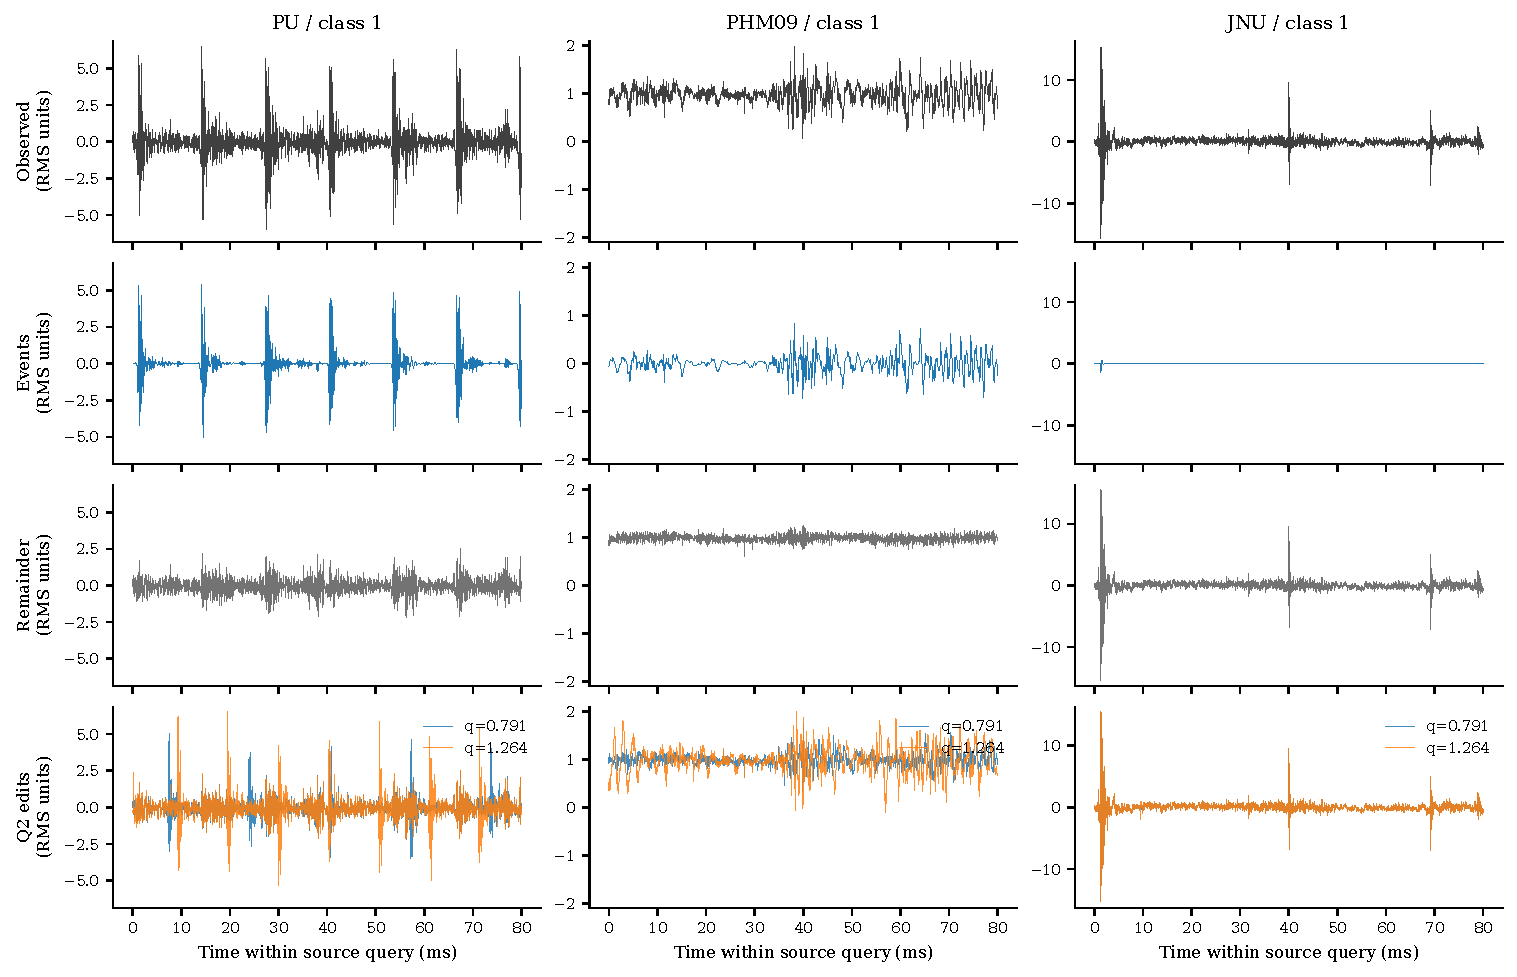
\includegraphics[width=.99\linewidth]{generated/real_source_edits.pdf}
\caption{Measured-source examples selected by the fixed metadata rule. Rows show
the observed query, estimated event component, retained remainder and two Q2
edits. Columns correspond to PU outer-race class, PHM09 configuration 2 and JNU
inner-race class. Time covers the entire registered query; all four rows in a
column share the same amplitude scale, divided by that observed query's RMS.
The weak estimated event in the selected JNU query is retained in the figure.}
\label{fig:source-edit}
\end{figure}

The examples show that the editor adapts its effective action to the estimated
event component. In the selected PU query, clear repeated transients enter the
event component and their locations change. The PHM09 example also retains a
substantial observation term. In the JNU example, most observed structure
remains in the remainder, so the edit is weak on this query. Neither the event
energy nor the remainder energy is interpreted as a separately measured
physical-factor share. Classification utility is assessed by the matched
experiments rather than by visually selecting a clean decomposition.
